\section{Implementation}
We have implemented the lens synthesis algorithm in $n$ lines of OCaml code.

\subsection{Synthesis Overview}
\begin{figure}
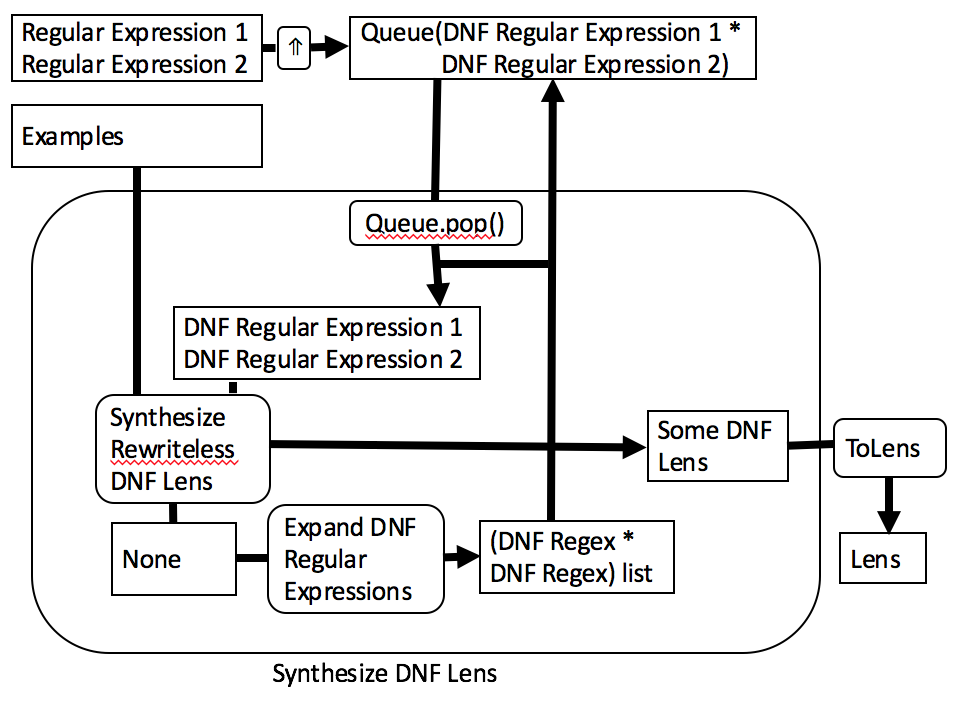
\includegraphics[scale=.5]{synth-lens-schematic.png}
\label{fig:synth-lens-schematic}
\end{figure}
The synthesis algorithm is shown in a schematic diagram in 
Figure~\ref{fig:synth-lens-schematic}.  The algorithm takes in a pair of
regular expressions, and examples, and converts the regular expressions into
DNF regular expressions, using \ToDNFRegex{}.
These then get enqueued, and SynthDNFLens, where the bulk of the work
occurs.

In SynthDNFLens, the highest priority DNF regular expression pair is popped.
Then, SynthRewritelessDNF sees if a DNF lens which satisfies the examples, which
does not include any applications of the rewrite rule, can be found.
If none are found, then each rewrite is applied once on each side of the regular
expressions.
This new list of DNF regular expression doubles is enqueued, and SynthDNFLens is
called again.
If one is found, this DNF lens gets converted to a normal lens, and is returned
to the user.

\subsection{Synthesis Algorithm}
\begin{lstlisting}[mathescape]


let gen_dnf_lens (q:priority_queue) (es:examples)
    : dnf_lens$_\bot$ =
  let (dnf_r,dnf_s,q) = q.pop()
  let dnf_lens_option =
    gen_tds_dnf_lens dnf_r dnf_s es in
  begin match 

let gen_lens (r:regex) (s:regex) (es:examples) : lens$_\bot$ =
  let dnf_r = $\ToDNFRegex$(r) in
  let dnf_s = $\ToDNFRegex$(s) in
  let dnf_lens = gen_dnf_lens(dnf_r, dnf_s, es) in
  to_lens(dnf_lens)
\end{lstlisting}
